\documentclass{beamer}
\usetheme{Boadilla}

\makeatother
\setbeamertemplate{footline}
{
    \leavevmode%
    \hbox{%
    \begin{beamercolorbox}[wd=.4\paperwidth,ht=2.25ex,dp=1ex,center]{author in head/foot}%
        \usebeamerfont{author in head/foot}\insertshortauthor
    \end{beamercolorbox}%
    \begin{beamercolorbox}[wd=.55\paperwidth,ht=2.25ex,dp=1ex,center]{title in head/foot}%
        \usebeamerfont{title in head/foot}\insertshorttitle
    \end{beamercolorbox}%
    \begin{beamercolorbox}[wd=.05\paperwidth,ht=2.25ex,dp=1ex,center]{date in head/foot}%
        \insertframenumber{}
    \end{beamercolorbox}}%
    \vskip0pt%
}
\makeatletter
\setbeamertemplate{navigation symbols}{}

\usepackage[T1]{fontenc}
\usepackage{lmodern}
\usepackage{amssymb,amsmath,bm,bbm}
\renewcommand{\familydefault}{\sfdefault}

\usepackage{mathtools}
\usepackage{graphicx}
\usepackage{threeparttable}
\usepackage{booktabs}
\usepackage{siunitx}
\sisetup{parse-numbers=false}

%\setlength{\OuterFrameSep}{-2pt}
%\makeatletter
%\preto{\@verbatim}{\topsep=-10pt \partopsep=-10pt }
%\makeatother

\title[Week 4:\ Logit Model]{Week 4:\ Logit Model}
\author[ResEcon 703:\ Advanced Econometrics]{ResEcon 703:\ Topics in Advanced Econometrics}
\date{Matt Woerman\\University of Massachusetts Amherst}

\begin{document}

{\setbeamertemplate{footline}{} 
\begin{frame}[noframenumbering]
    \titlepage
\end{frame}
}

\begin{frame}\frametitle{Agenda}
    Last week
    \begin{itemize}
        \item Random utility model
    \end{itemize}
    \vspace{2ex}
    Today
    \begin{columns}
        \begin{column}{0.5\textwidth}
            \begin{itemize}
                \item \hyperlink{page.\getpagerefnumber{logit}}{Logit model}
                \item \hyperlink{page.\getpagerefnumber{probs}}{Logit choice probabilities}
                \item \hyperlink{page.\getpagerefnumber{binary}}{Binary logit model}
                \item \hyperlink{page.\getpagerefnumber{multi}}{Multinomial logit model}
                \item \hyperlink{page.\getpagerefnumber{marginal}}{Marginal effects and elasticities}
                \item \hyperlink{page.\getpagerefnumber{subs}}{Logit substitution patterns}
            \end{itemize}
        \end{column}
        \begin{column}{0.5\textwidth}
            \begin{itemize}
                \item \hyperlink{page.\getpagerefnumber{params}}{Properties of logit parameters}
                \item \hyperlink{page.\getpagerefnumber{counter}}{Counterfactuals and welfare}
                \item \hyperlink{page.\getpagerefnumber{empirical}}{Empirical considerations}
                \item \hyperlink{page.\getpagerefnumber{binary_r}}{Binary logit model R example}
                \item \hyperlink{page.\getpagerefnumber{multi_r}}{Multinomial logit model R example}
            \end{itemize}
            \vspace{\fill}
        \end{column}
    \end{columns}
    \vspace{3ex}
    This week's reading
    \begin{itemize}
        \item Train textbook, chapters 3.1--3.6
    \end{itemize}
\end{frame}

\section{Logit Model}
\label{logit}
\begin{frame}\frametitle{}
    \vfill
    \centering
    \begin{beamercolorbox}[center]{title}
        \Large Logit Model
    \end{beamercolorbox}
    \vfill
\end{frame}

\begin{frame}\frametitle{Random Utility Model Recap}
    A decision maker chooses the alternative that maximizes utility
    \begin{itemize}
		\item A decision maker, $n$, faces a choice among $J$ discrete alternatives
    	\item Alternative $j$ provides utility $U_{nj}$ (where $j = 1, \ldots, J$)
    	\item $n$ chooses $i$ if and only if $U_{ni} > U_{nj} \; \forall j \neq i$
   	\end{itemize}
   	\vspace{2ex}
   	We (the econometricians) do not observe utility $U_{nj}$, so we model it as being composed of
   	\begin{itemize}
		\item $V_{nj}$: Utility from observed attributes 
		\item $\varepsilon_{nj}$: Utility from unobserved attributes, which we treat as random
	\end{itemize}
	$$U_{nj} = V_{nj} + \varepsilon_{nj}$$ \\
	\vspace{2ex}
	The probability that decision maker $n$ chooses alternative $i$ is
    \begin{align*}
    	P_{ni} & = \Pr(U_{ni} > U_{nj} \; \forall j \neq i) \\
    	& = \int_{\bm{\varepsilon}} \mathbbm{1}(\varepsilon_{nj} - \varepsilon_{ni} < V_{ni} - V_{nj} \; \forall j \neq i) f(\bm{\varepsilon}_n) d\bm{\varepsilon}_n
    \end{align*}
\end{frame}

\begin{frame}\frametitle{Logit Model}
    The logit model makes a simple (but sometimes overly strong) assumption about the joint density of unobserved utility, $f(\bm{\varepsilon}_n)$
    $$\varepsilon_{nj} \sim \text{i.i.d.\ type I extreme value (Gumbel) with } Var(\varepsilon_{nj}) = \frac{\pi^2}{6}$$ \\
    \vspace{3ex}
    Why make this assumption about the unobserved component of utilities?
    \begin{itemize}
    	\item It yields a simple closed-form expression for choice probabilities
    \end{itemize}
    \vspace{3ex}
    Are there any downsides to making this assumption?
    \begin{itemize}
    	\item It implies substitution patterns that may be unrealistic
    \end{itemize}
\end{frame}

\begin{frame}\frametitle{Type I Extreme Value Density and Distribution}
    Type I extreme value is similar to a normal distribution but with a fatter tail on one side \\
    \begin{columns}
		\begin{column}{0.5\textwidth}
			\begin{center}
				Probability density
				$$f(\varepsilon_{nj}) = e^{-\varepsilon_{nj}} e^{-e^{-\varepsilon_{nj}}}$$
				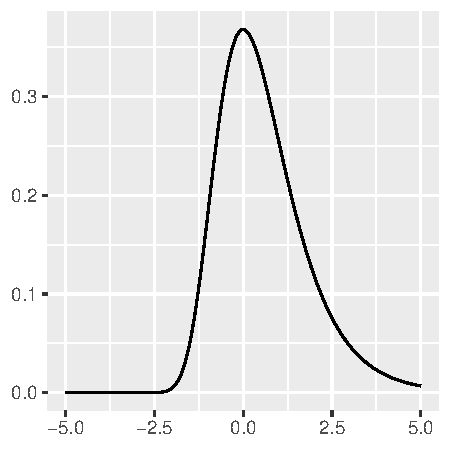
\includegraphics[width=0.8\textwidth]{ev_pdf.pdf}      
			\end{center}
		\end{column}
		\begin{column}{0.5\textwidth}
    		\begin{center}
     			Cumulative distribution 
     			$$F(\varepsilon_{nj}) = e^{-e^{-\varepsilon_{nj}}}$$
				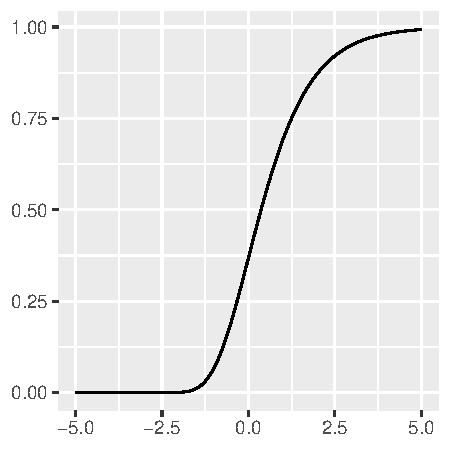
\includegraphics[width=0.8\textwidth]{ev_cdf.pdf}          
     		\end{center}
		\end{column}
	\end{columns}
\end{frame}

\begin{frame}\frametitle{Logistic Density and Distribution}
    The difference of two type I extreme value draws, $\varepsilon_{nji}^* = \varepsilon_{nj} - \varepsilon_{ni}$, follows the logistic distribution
    \begin{columns}
		\begin{column}{0.5\textwidth}
			\begin{center}
				Probability density \\
				\vspace{-4ex}
				$$f(\varepsilon_{nji}^*) = \frac{e^{\varepsilon_{nji}^*}}{\left( 1 + e^{\varepsilon_{nji}^*} \right)^2}$$ \\
				\vspace{-2ex}
				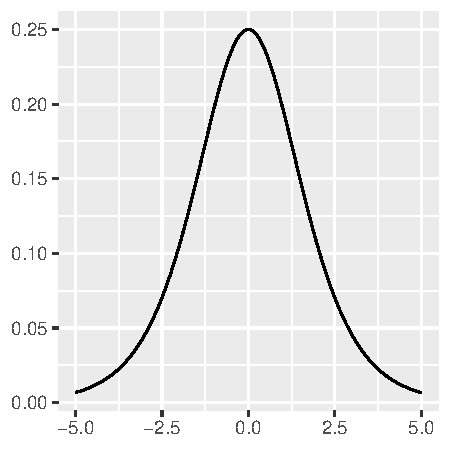
\includegraphics[width=0.8\textwidth]{logistic_pdf.pdf}      
			\end{center}
		\end{column}
		\begin{column}{0.5\textwidth}
    		\begin{center}
     			Cumulative distribution \\
     			\vspace{-4ex}
     			$$F(\varepsilon_{nji}^*) = \frac{e^{\varepsilon_{nji}^*}}{1 + e^{\varepsilon_{nji}^*}}$$ \\
     			\vspace{0ex}
				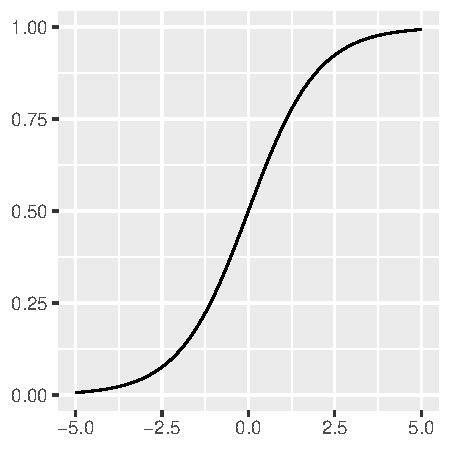
\includegraphics[width=0.8\textwidth]{logistic_cdf.pdf}          
     		\end{center}
		\end{column}
	\end{columns}
\end{frame}

\section{Logit Choice Probabilities}
\label{probs}
\begin{frame}\frametitle{}
    \vfill
    \centering
    \begin{beamercolorbox}[center]{title}
        \Large Logit Choice Probabilities
    \end{beamercolorbox}
    \vfill
\end{frame}

\begin{frame}\frametitle{Logit Choice Probabilities}
	\vspace{-4ex}
    \begin{align*}
    	P_{ni} & = \Pr(U_{ni} > U_{nj} \; \forall j \neq i) \\
    	& = \Pr(V_{ni} + \varepsilon_{ni} > V_{nj} + \varepsilon_{nj} \; \forall j \neq i) \\
    	& = \Pr(\varepsilon_{nj} < \varepsilon_{ni} + V_{ni} - V_{nj} \; \forall j \neq i)
    \end{align*} \\
    \vspace{1ex}
    Suppose we know $V_{ni}$, $V_{nj}$, and $\varepsilon_{ni}$
    \begin{itemize}
        \item We known the right-hand side of the inequality inside the probability
    \end{itemize}
    \vspace{2ex}
    For a single $\varepsilon_{nj}$, this probability is the cumulative distribution of a type I extreme value random variable
    $$\Pr(\varepsilon_{nj} < \varepsilon_{ni} + V_{ni} - V_{nj} \mid \varepsilon_{ni}) = e^{-e^{-(\varepsilon_{ni} + V_{ni} - V_{nj})}}$$
    We need to know this probability $\forall j \neq i$, not just a single $j$
    \begin{itemize}
        \item $\varepsilon_{nj}$ is i.i.d., so we can take the product of the probability for each $\varepsilon_{nj}$
    \end{itemize}
    $$P_{ni} \mid \varepsilon_{ni} = \prod_{j \neq i} e^{-e^{-(\varepsilon_{ni} + V_{ni} - V_{nj})}}$$
\end{frame}

\begin{frame}\frametitle{Logit Choice Probabilities}
    Conditional on knowing $\varepsilon_{ni}$, the choice probability of alternative $i$ is
    $$P_{ni} \mid \varepsilon_{ni} = \prod_{j \neq i} e^{-e^{-(\varepsilon_{ni} + V_{ni} - V_{nj})}}$$ \\
    But $\varepsilon_{ni}$ is random, so we have to integrate over the density of $\varepsilon_{ni}$
    \begin{align*}
        P_{ni} & = \int \left( \prod_{j \neq i} e^{-e^{-(\varepsilon_{ni} + V_{ni} - V_{nj})}} \right) e^{-\varepsilon_{ni}} e^{-e^{-\varepsilon_{ni}}} d\varepsilon_{ni} \\
        & = \frac{e^{V_{ni}}}{\sum_j e^{V_{nj}}}
    \end{align*} \\
    \vspace{-1ex}
    \begin{itemize}
        \item See the textbook for the proof of this equivalence
    \end{itemize}
    \vspace{2ex}
    The probability of $n$ choosing $i$ is a closed-form expression that depends on the representative utility (or observable attributes) of all alternatives
\end{frame}

\begin{frame}\frametitle{Properties of Logit Choice Probabilities}
    $P_{ni}$ is always within the range $(0, 1)$
    \begin{itemize}
        \item $P_{ni} \rightarrow 1$ as $V_{ni} \rightarrow \infty$
        \item $P_{ni} \rightarrow 0$ as $V_{ni} \rightarrow -\infty$
    \end{itemize}
    \vspace{2ex}
    Choice probabilities sum to 1
    $$\sum_{i = 1}^J P_{ni} = \sum_{i = 1}^J \frac{e^{V_{ni}}}{\sum_j e^{V_{nj}}} =\frac{\sum_i e^{V_{ni}}}{\sum_j e^{V_{nj}}} = 1$$ \\
    \vspace{2ex}
    Choice probability is a sigmoidal function of representative utility (see the logistic CDF)
    \begin{itemize}
        \item Marginal effects are small when probabilities are close to 0 or 1
        \item Marginal effects are largest when $P_{ni} = 0.5$
    \end{itemize}
\end{frame}

\begin{frame}\frametitle{Linear Representative Utility}
    If we assume representative utility is linear in parameters
    $$V_{nj} = \bm{\beta}' \bm{x}_{nj}$$ \\
    then the logit choice probability is
    $$P_{ni} = \frac{e^{\bm{\beta}' \bm{x}_{ni}}}{\sum_j e^{\bm{\beta}' \bm{x}_{nj}}}$$ \\
    \vspace{2ex}
    Reminders about parameters and estimation
    \begin{itemize}
        \item With linear representative utility, the structural parameters will typically give us the marginal utility of attributes, characteristics, etc.
        \begin{itemize}
            \item We can use different models of representative utility to get different structural parameters
        \end{itemize}
    	\item We want to find the parameter values that make choice probabilities consistent with observed choices
    \end{itemize}
\end{frame}

\section{Binary Logit Model}
\label{binary}
\begin{frame}\frametitle{}
    \vfill
    \centering
    \begin{beamercolorbox}[center]{title}
        \Large Binary Logit Model
    \end{beamercolorbox}
    \vfill
\end{frame}

\begin{frame}\frametitle{Binary Logit Choice Probabilities}
	Under the logit assumption, choice probabilities for a binary choice are
	\vspace{-1ex}
	\begin{align*}
		P_{n1} & = \frac{e^{V_{n1}}}{e^{V_{n1}} + e^{V_{n2}}} \\
		P_{n2} & = \frac{e^{V_{n2}}}{e^{V_{n1}} + e^{V_{n2}}}
	\end{align*} \\
	\vspace{-1ex}
    \begin{itemize}
    	\item There are several alternate ways to express these choice probabilities
    \end{itemize}
    \vspace{2ex}
    A more succinct expression for the choice probability of alternative 1 is
    \begin{align*}
    	P_{n1} & = \frac{1}{1 + e^{-(V_{n1} - V_{n2})}}
    	\intertext{If we assume representative utility is linear, $V_{nj} = \bm{\beta}' \bm{x}_{nj}$}
		P_{n1} & = \frac{1}{1 + e^{-\bm{\beta}' (\bm{x}_{n1} - \bm{x}_{n2})}}
	\end{align*}
	But this choice probability is nonlinear, so we cannot use OLS
\end{frame}

\begin{frame}\frametitle{Binary Logit Odds Ratio}
    We can instead calculate the odds ratio of alternative 1
    \begin{align*}
   		\frac{P_{n1}}{1 - P_{n1}} & = \frac{P_{n1}}{P_{n2}} = e^{V_{n1} - V_{n2}}
   		\intertext{Then the log odds ratio of alternative 1 is}
    	\ln \left( \frac{P_{n1}}{1 - P_{n1}} \right) & = V_{n1} - V_{n2}
    	\intertext{If we assume representative utility is linear, $V_{nj} = \bm{\beta}' \bm{x}_{nj}$}
    	\ln \left( \frac{P_{n1}}{1 - P_{n1}} \right) & = \bm{\beta}' (\bm{x}_{n1} - \bm{x}_{n2})
    	\intertext{We might express this log odds ratio more generally as}
    	\ln \left( \frac{P_{n1}}{1 - P_{n1}} \right) & = \bm{\beta}' \bm{x}_{n}
    \end{align*}
    where $\bm{x}_n = \{ \bm{x}_{n1}, \bm{x}_{n2} \}$ contains data about both alternatives
\end{frame}

\begin{frame}\frametitle{Binary Logit Estimation in R}
	The log odds ratio for the binary logit model is
    $$\ln \left( \frac{P_{n1}}{1 - P_{n1}} \right) = \bm{\beta}' \bm{x}_{n}$$ \\
    \vspace{2ex}
    Now we have an expression with a linear right-hand side, but the left-hand side is nonlinear!
    \begin{itemize}
    	\item This model is part of the family known as ``generalized linear models''
    	\item We can estimate this model in R using the \texttt{glm()} function with the argument \texttt{family = "binomial"}
    \end{itemize}
    \vspace{2ex}
    This only works for a binary logit model because it is implicitly a single comparison that can be fully represented with one equation
    \begin{itemize}
    	\item Estimation gets more complicated with more than two alternatives
    \end{itemize}
\end{frame}

\begin{frame}\frametitle{Binary Logit Example}
    A person chooses whether to take a car ($c$) or a bus ($b$) to work
    \begin{itemize}
        \item We observe the time, $T$, and cost, $M$, of each alternative
    \end{itemize}
    \vspace{2ex}
    We specify the representative utility of each alternative as
    $$V_{nj} = \beta_{0j} + \beta_1 T_{nj} + \beta_2 M_{nj}$$ \\
    \vspace{1ex}
    Under the logit assumption, the choice probability of driving is
    \begin{align*}
        P_{nc} & = \frac{e^{\beta_{0c} + \beta_1 T_{nc} + \beta_2 M_{nc}}}{e^{\beta_{0c} + \beta_1 T_{nc} + \beta_2 M_{nc}} + e^{\beta_{0b} + \beta_1 T_{nb} + \beta_2 M_{nb}}} \\
        & = \frac{1}{1 + e^{-(\beta_{0c} - \beta_{ob}) - \beta_1 (T_{nc} - T_{ncb}) - \beta_2 (M_{nc} - M_{nb})}} 
    \end{align*} \\
    \vspace{1ex}
    The log odds ratio of driving is
    $$\ln \left( \frac{P_{nc}}{1 - P_{nc}} \right) = (\beta_{0c} - \beta_{0b}) + \beta_1 (T_{nc} - T_{nb}) + \beta_2 (M_{nc} - M_{nb})$$
\end{frame}

\section{Multinomial Logit Model}
\label{multi}
\begin{frame}\frametitle{}
    \vfill
    \centering
    \begin{beamercolorbox}[center]{title}
        \Large Multinomial Logit Model
    \end{beamercolorbox}
    \vfill
\end{frame}

\begin{frame}\frametitle{Multinomial Logit Model}
    With a multinomial discrete choice (more than two alternatives), the problem becomes more complicated
    \begin{itemize}
        \item We cannot reduce the choice down to one choice probability
    \end{itemize}
    \vspace{2ex}
    Under the logit assumption, the choice probabilities of the alternatives are
    \begin{align*}
        P_{n1} & = \frac{e^{V_{n1}}}{e^{V_{n1}} + e^{V_{n2}} + \cdots + e^{V_{nJ}}} \\
        P_{n2} & = \frac{e^{V_{n2}}}{e^{V_{n1}} + e^{V_{n2}} + \cdots + e^{V_{nJ}}} \\
        & \vdotswithin{=} \\
        P_{nJ} & = \frac{e^{V_{nJ}}}{e^{V_{n1}} + e^{V_{n2}} + \cdots + e^{V_{nJ}}}
    \end{align*}
\end{frame}

\begin{frame}\frametitle{Multinomial Logit Estimation in R}
    \vspace{-3ex}
    \begin{align*}
        P_{ni} & = \frac{e^{V_{ni}}}{\sum_j e^{V_{nj}}}
        \intertext{If we assume representative utility is linear, $V_{nj} = \bm{\beta}' \bm{x}_{nj}$}
        P_{ni} & = \frac{e^{\bm{\beta}' \bm{x}_{ni}}}{\sum_j e^{\bm{\beta}' \bm{x}_{nj}}}
    \end{align*} \\
    \vspace{1ex}
    We will use the \texttt{mlogit} package in R to estimate multinomial logit models
    \begin{itemize}
        \item Find the values of the structural parameters that make choice probabilities consistent with observed choices
    \end{itemize}
    \vspace{2ex}
    The \texttt{mlogit} package requires us to
    \begin{enumerate}
        \item Organize the data to identify decision makers and alternatives
        \item Specify the formula for representative utility
    \end{enumerate}
\end{frame}

\section{Marginal Effects and Elasticities}
\label{marginal}
\begin{frame}\frametitle{}
    \vfill
    \centering
    \begin{beamercolorbox}[center]{title}
        \Large Marginal Effects and Elasticities
    \end{beamercolorbox}
    \vfill
\end{frame}

\begin{frame}\frametitle{Marginal Effects}
    Unlike a linear probability model, the structural parameters of a logit model cannot be interpreted as marginal effects on probability
    \begin{itemize}
     	\item But we can use the choice probabilities and parameters to derive the marginal effects!
    \end{itemize}
    \vspace{2ex}
    The marginal effect of $z_{ni}$, an observed attribute of alternative $i$, on $P_{ni}$ is
    \begin{align*}
    	\frac{\partial P_{ni}}{\partial z_{ni}} & = \frac{\partial \left( e^{V_{ni}} / \sum_j e^{V_{nj}} \right)}{\partial z_{ni}} \\
    	& = \frac{\partial V_{ni}}{\partial z_{ni}} P_{ni} (1 - P_{ni}) \\
    	\intertext{If $V_{ni}$ is linear in $z_{ni}$ with coefficient $\beta_z$, then the marginal effect is}
    	\frac{\partial P_{ni}}{\partial z_{ni}} & = \beta_z P_{ni} (1 - P_{ni})
    \end{align*}
\end{frame}

\begin{frame}\frametitle{Cross Marginal Effects}
    The marginal effect of $z_{nj}$, an observed attribute of alternative $j$, on $P_{ni}$ is
    \begin{align*}
    	\frac{\partial P_{ni}}{\partial z_{nj}} & = \frac{\partial \left( e^{V_{ni}} / \sum_k e^{V_{nk}} \right)}{\partial z_{nj}} \\
    	& = -\frac{\partial V_{nj}}{\partial z_{nj}} P_{ni} P_{nj} \\
    	\intertext{If $V_{nj}$ is linear in $z_{nj}$ with coefficient $\beta_z$, then the marginal effect is}
    	\frac{\partial P_{ni}}{\partial z_{nj}} & = -\beta_z P_{ni} P_{nj}
    \end{align*} \\
    \vspace{2ex}
    In a binary logit model, these marginal effect expressions are negatives of each another
\end{frame}

\begin{frame}\frametitle{Elasticities}
    Sometimes elasticities are more informative than marginal effects
        \begin{itemize}
            \item Percent changes rather than level changes
        \end{itemize}
    \vspace{3ex}
    The elasticity of $P_{ni}$ with respect to $z_{ni}$, an observed attribute of alternative $i$, is
    \begin{align*}
    	E_{iz_{ni}} & = \frac{\partial P_{ni}}{\partial z_{ni}} \frac{z_{ni}}{P_{ni}} \\
    	& = \frac{\partial V_{ni}}{\partial z_{ni}} z_{ni} (1 - P_{ni}) \\
    	\intertext{If $V_{ni}$ is linear in $z_{ni}$ with coefficient $\beta_z$, then the elasticity is}
    	E_{iz_{ni}} & = \beta_z z_{ni} (1 - P_{ni})
    \end{align*}
\end{frame}

\begin{frame}\frametitle{Cross Elasticities}
    The elasticity of $P_{ni}$ with respect to $z_{nj}$, an observed attribute of alternative $j$, is
    \begin{align*}
    	E_{iz_{nj}} & = \frac{\partial P_{ni}}{\partial z_{nj}} \frac{z_{nj}}{P_{ni}} \\
    	& = -\frac{\partial V_{nj}}{\partial z_{nj}} z_{nj} P_{nj} \\
    	\intertext{If $V_{nj}$ is linear in $z_{nj}$ with coefficient $\beta_z$, then the elasticity is}
    	E_{iz_{nj}} & = -\beta_z z_{nj} P_{nj}
    \end{align*} \\
    \vspace{2ex}
    The cross-elasticity of $P_{ni}$ with respect to $z_{nj}$ depends only on attributes of alternative $j$ and not on alternative $i$
\end{frame}

\section{Logit Substitution Patterns}
\label{subs}
\begin{frame}\frametitle{}
    \vfill
    \centering
    \begin{beamercolorbox}[center]{title}
        \Large Logit Substitution Patterns
    \end{beamercolorbox}
    \vfill
\end{frame}

\begin{frame}\frametitle{Independence of Irrelevant Alternatives}
    The ratio of any two logit choice probabilities is
    $$\frac{P_{ni}}{P_{nk}} = \frac{e^{V_{ni}}}{e^{V_{nk}}}$$
    This ratio only depends on attributes of alternatives $i$ and $k$, so the relative probability of choosing $i$ over $k$ is considered to be independent of irrelevant alternatives (IIA) \\
    \vspace{2ex}
    When IIA holds, you can estimate consistent parameters using only a subset of alternatives for each decision maker
    \begin{itemize}
        \item When the choice set is too large to be computationally feasible, you only have to consider a subset of alternatives
        \item When you only care about a subset of the choice set, you can ignore decision makers who choose the other alternatives
    \end{itemize}
    \vspace{2ex}
    But there is one major downside to the IIA property
\end{frame}

\begin{frame}\frametitle{Red-Bus/Blue-Bus Problem}
    Two travel modes to commute to work: car and blue bus
    \begin{itemize}
        \item For simplicity, assume choice probabilities are equal
    \end{itemize}
    $$P_c = P_{bb} = \frac{1}{2} \quad \Rightarrow \quad \frac{P_c}{P_{bb}} = 1$$ \\
    Now suppose a red bus is introduced with all attributes identical to the blue bus except the color
    \begin{itemize}
        \item Assuming the commuter does not care about the color of the bus
    \end{itemize}
    $$P_{rb} = P_{bb} \quad \Rightarrow \quad \frac{P_{rb}}{P_{bb}} = 1$$ \\
    But from the IIA property, the ratio of car and blue bus is not changed by the introduction of the red bus
    \begin{itemize}
        \item The choice probability for all three modes must be equal
    \end{itemize}
    $$P_c = P_{bb} = P_{rb} = \frac{1}{3}$$
    Should the introduction of a red bus change the probability of driving?
\end{frame}

\begin{frame}\frametitle{Proportional Substitution}
    The cross-elasticity of $P_{ni}$ with respect to $z_{nj}$ is given by (assuming linearity of representative utility)
    $$E_{iz_{nj}} = -\beta_z z_{nj} P_{nj}$$
    This cross-elasticity depends only on attributes of alternative $j$ and not on alternative $i$
    \begin{itemize}
        \item This cross-elasticity is the same for every alternative other than $j$!
    \end{itemize}
    \vspace{2ex}
    When an attribute of one alternative changes, all other choice probabilities are changed by the same percentage (not percentage points)
    \begin{itemize}
        \item That is, substitution to other alternatives is proportional to their original choice probabilities
    \end{itemize}
\end{frame}

\begin{frame}\frametitle{Proportional Substitution Example}
    \begin{columns}
        \begin{column}{0.333\textwidth}
            \centering
            
\includegraphics[width=\textwidth]{hummer.jpg}
        \end{column}
        \begin{column}{0.333\textwidth}
            \centering
            
\includegraphics[width=0.95\textwidth]{escalade.jpg}
        \end{column}
        \begin{column}{0.333\textwidth}
            \centering
            
\includegraphics[width=0.65\textwidth]{smart.png}
        \end{column}
    \end{columns}
    \begin{columns}
        \begin{column}{0.333\textwidth}
            \centering Hummer H2
        \end{column}
        \begin{column}{0.333\textwidth}
            \centering Cadillac Escalade
        \end{column}
        \begin{column}{0.333\textwidth}
            \centering Smart Pure EV
        \end{column}
    \end{columns}
    \vspace{3ex}
    Suppose Hummer lowers the price of the H2
    \begin{itemize}
        \item Will that attract a greater proportion of Escalade drivers or Pure EV drivers?
        \item The logit model says that substitution to the H2 will be proportionally equal for these very different vehicles!
    \end{itemize}
\end{frame}

\section{Properties of Logit Parameters}
\label{params}
\begin{frame}\frametitle{}
    \vfill
    \centering
    \begin{beamercolorbox}[center]{title}
        \Large Properties of Logit Parameters
    \end{beamercolorbox}
    \vfill
\end{frame}

\begin{frame}\frametitle{Variation in Preferences}
    A decision maker's preferences can vary for many reasons, some of which are observable, but others are not
    \begin{itemize}
    	\item The logit model can only explicitly capture variation due to observable attributes
        \item Future models will allow for unobservable variation
    \end{itemize}
    \vspace{1ex}
    Consider some sources of preference variation in the car-or-bus commute choice
    \begin{itemize}
    	\item Some people hate driving and some people love it, but we do not directly observe this preference
    	\begin{itemize}
    		\item We cannot include this variation in the logit model
    	\end{itemize}
    	\item People with higher incomes care less about the cost of each alternative
    \end{itemize}
    $$\beta_n = \frac{\beta}{I_n} \quad \Rightarrow \quad U_{nc} = \alpha T_{nc} + \beta \frac{M_{nc}}{I_n} + \varepsilon_{nc}$$ \\
    \vspace{1ex}
    The logit model allows for parameters to be a function of observable data
\end{frame}

\begin{frame}\frametitle{Scale Parameter}
    In the logit model, we assume the unobserved and random component of utility has variance $\pi^2 / 6$
    \begin{itemize}
    	\item This assumption may seem restrictive, but we can use a scale parameter, $\sigma$, to allow for a different variance \\
    \end{itemize}
    \vspace{2ex}
    Suppose the random utility, $\varepsilon_{nj}^*$, actually has variance $\sigma^2 \times (\pi^2 / 6)$
    $$U_{nj}^* = V_{nj} + \varepsilon_{nj}^*$$
    Dividing by $\sigma$ gives a scaled model
    $$U_{nj} = \frac{V_{nj}}{\sigma} + \varepsilon_{nj} \text{ where } \varepsilon_{nj} = \frac{\varepsilon_{nj}^*}{\sigma}$$
    The variance of the scaled random utility is
    $$Var(\varepsilon_{nj}) = \frac{1}{\sigma^2} Var(\varepsilon_{nj}^*) = \frac{\pi^2}{6}$$
\end{frame}

\begin{frame}\frametitle{Logit Choice Probabilities with a Scale Parameter}
    In the scaled model, choice probabilities are
    \begin{align*}
    P_{ni} & = \frac{e^{V_{ni} / \sigma}}{\sum_j e^{V_{nj} / \sigma}} \\
    \intertext{If $V_{nj}$ is linear in parameters with coefficients $\bm{\beta}^*$}
    P_{ni} & = \frac{e^{(\bm{\beta}^* / \sigma)' \bm{x}_{ni}}}{\sum_j e^{(\bm{\beta}^* / \sigma)' \bm{x}_{nj}}}
    \intertext{But $\bm{\beta}^*$ and $\sigma$ are not separately identified, so we can only estimate their ratio, $\bm{\beta} = \bm{\beta}^* / \sigma$, which gives the standard logit expression}
    P_{ni} & = \frac{e^{\bm{\beta}' \bm{x}_{ni}}}{\sum_j e^{\bm{\beta}' \bm{x}_{nj}}}
    \end{align*}
    Parameters are estimated relative to the variance of unobserved utility
\end{frame}

\begin{frame}\frametitle{Heteroskedasticity and the Scale Parameter}
    Different subsets of decision makers may each have a different variance of random utility
    \begin{itemize}
    	\item We can use scale parameters to account for this groupwise heteroskedasticity
    	\item We can estimate the relative scale parameters of each group compared to one reference group
    \end{itemize}
    \vspace{2ex}
    Suppose we have commute data for both Amherst ($A$) and Boston ($B$)
    \begin{itemize}
    	\item The scale parameters for each city are $\sigma^A$ and $\sigma^B$ with $k = (\sigma^B / \sigma^A)^2$
    \end{itemize}
    \begin{align*}
    	\text{Amherst:}& \quad P_{ni} = \frac{e^{\bm{\beta}' \bm{x}_{ni}}}{\sum_j e^{\bm{\beta}' \bm{x}_{nj}}} \\
    	\text{Boston:}& \quad P_{ni} = \frac{e^{(\bm{\beta} / \sqrt{k})' \bm{x}_{ni}}}{\sum_j e^{(\bm{\beta} / \sqrt{k})' \bm{x}_{nj}}}
    \end{align*}
\end{frame}

\section{Counterfactuals and Welfare}
\label{counter}
\begin{frame}\frametitle{}
    \vfill
    \centering
    \begin{beamercolorbox}[center]{title}
        \Large Counterfactuals and Welfare
    \end{beamercolorbox}
    \vfill
\end{frame}

\begin{frame}\frametitle{Counterfactual Simulations}
    An advantage of a structural econometric model is the ability to conduct counterfactual simulations and calculate their welfare consequences \\
    \vspace{2ex}
    You can compare outcomes in the observed empirical setting to outcomes in an alternate setting with some aspect manipulated
    \begin{itemize}
        \item Different attributes or data
        \item Different choice set
        \item Different structural parameters
    \end{itemize}
    \vspace{2ex}
    Examples of counterfactual simulations
    \begin{itemize}
        \item Estimate the demand for education in order to simulate the effects of a school voucher program
        \item Estimate how farmers choose which crop to plant in order to simulate the effects of a groundwater sustainability policy
        \item Estimate the supply of labor in order to simulate the effects of an income tax change
    \end{itemize}
\end{frame}

\begin{frame}\frametitle{Simulating Individual Choices in the Logit Model}
    We cannot simulate discrete choices with certainty, but we can use choice probabilities to simulate choices in expectation
    $$E(Y_{ni}) = P_{ni} = \frac{e^{V_{ni}}}{\sum_j e^{V_{nj}}}$$
    where $Y_{ni} = 1$ if and only if $n$ chooses $i$ \\
    \vspace{3ex}
    The change in the expectation of a decision maker's choice due to a change in the choice setting is
    $$\Delta E(Y_{ni}) = P_{ni}^1 - P_{ni}^0 = \frac{e^{V_{ni}^1}}{\sum_{j = 1}^{J^1} e^{V_{nj}^1}} - \frac{e^{V_{ni}^0}}{\sum_{j = 1} ^{J^0} e^{V_{nj}^0}}$$
    where the 1 superscript denotes the counterfactual and the 0 superscript denotes the observed empirical setting
    \begin{itemize}
        \item Note: You must ``simulate'' choices in the original setting!
    \end{itemize}
\end{frame}

\begin{frame}\frametitle{Simulating Aggregate Choices in the Logit Model}
    We can simulate the aggregate number of decision makers expected to choose alternative $i$, which we denote $A_i$, by summing the individual expectation over all agents
    $$E(A_i) = \sum_{n = 1}^N E(Y_{ni}) = \sum_{n = 1}^N P_{ni}$$ \\
    \vspace{2ex}
    The expected change in the aggregate number of decision makers choosing alternative $i$ due to a change in the choice setting is
    $$\Delta E(A_i) = \sum_{n = 1}^N P_{ni}^1 - \sum_{n = 1}^N P_{ni}^0 = \sum_{n = 1}^N \frac{e^{V_{ni}^1}}{\sum_{j = 1}^{J^1} e^{V_{nj}^1}} - \sum_{n = 1}^N \frac{e^{V_{ni}^0}}{\sum_{j = 1} ^{J^0} e^{V_{nj}^0}}$$
    \begin{itemize}
        \item Reminder: You must ``simulate'' choices in the original setting!
    \end{itemize}
\end{frame}

\begin{frame}\frametitle{Consumer Surplus}
    The logit model gives a closed-form expression for consumer surplus 
    \begin{itemize}
        \item Monetary gain to a consumer from ``purchasing'' a good for less than the value the consumer places on the good
    \end{itemize}
    \vspace{2ex}
    If we know the marginal utility of income for decision maker $n$, which we denote $\alpha_n$, then the consumer surplus from a choice setting is
    \begin{align*}
        CS_n & = \frac{1}{\alpha_n} \max_j (U_{nj}) \\
        \intertext{We do not observe $U_{nj}$, but we know it in expectation}
        E(CS_n) & = \frac{1}{\alpha_n} E\left[ \max_j (V_{nj} + \varepsilon_{nj}) \right] \\
        \intertext{If we further assume utility is linear in income, we get}
        E(CS_n) & = \frac{1}{\alpha_n} \ln \left( \sum_{j = 1}^J e^{V_{nj}} \right) + C
    \end{align*}
    \vspace{-1ex}
\end{frame}

\begin{frame}\frametitle{Consumer Surplus in Counterfactuals}
    The expected consumer surplus that decision maker $n$ obtains when faced with a choice setting is
    $$E(CS_n) = \frac{1}{\alpha_n} \ln \left( \sum_{j = 1}^J e^{V_{nj}} \right) + C$$ \\
    \vspace{2ex}
    The expected change in consumer surplus due to a change in the choice setting is
    $$\Delta E(CS_n) = \frac{1}{\alpha_n} \left[ \ln \left( \sum_{j = 1}^{J^1} e^{V_{nj}^1} \right) - \ln \left( \sum_{j = 1}^{J^0} e^{V_{nj}^0} \right) \right]$$
    \begin{itemize}
        \item Reminder: You must ``simulate'' consumer surplus in the original setting!
    \end{itemize}
\end{frame}

\section{Empirical Considerations}
\label{empirical}
\begin{frame}\frametitle{}
    \vfill
    \centering
    \begin{beamercolorbox}[center]{title}
        \Large Empirical Considerations
    \end{beamercolorbox}
    \vfill
\end{frame}

\begin{frame}\frametitle{Market-Level Data}
    The logit model can be (and often is) estimated from market-level data
    \begin{itemize}
        \item You observe the price, market share, and attributes of every cereal brand at the grocery store, and you want to estimate the structural parameters of consumer decision making that explain those purchases
    \end{itemize}
    \vspace{1ex}
    When aggregated over many consumers, choice probabilities become market shares
    $$S_i = \frac{e^{V_{i}}}{\sum_j e^{V_j}}$$
    If we assume representative utility is liner, $V_j = \bm{\beta}' \bm{x}_j$
    $$\ln(S_i) - \ln(S_j) = \bm{\beta}' (\bm{x}_i - \bm{x}_j)$$
    Set one alternative to be your reference (usually the outside option) and estimate the linear regression for the other $J - 1$ alternatives
    $$\ln(S_i) - \ln(S_0) = \bm{\beta}' (\bm{x}_i - \bm{x}_0) + \omega_i$$
\end{frame}

\begin{frame}\frametitle{Panel Data}
    If we observe panel data for a discrete choice problem, we can add a time index to our random utility model and logit choice probabilities
    $$U_{njt} = V_{njt} + \varepsilon_{njt} \quad \Rightarrow \quad P_{nit} = \frac{e^{V_{nit}}}{\sum_j e^{V_{njt}}}$$ \\
    \vspace{2ex}
    We can estimate this model just as in the cross-section
    \begin{itemize}
        \item We can include lagged or future variables to capture ``dynamics''
        \item We can include previous choices as explanatory variables to represent behavioral factors like habit formation
    \end{itemize}
    \vspace{2ex}
    The logit assumption still has to hold
    $$\varepsilon_{njt} \sim \text{i.i.d.\ type I extreme value (Gumbel) with } Var(\varepsilon_{njt}) = \frac{\pi^2}{6}$$ \\
    \begin{itemize}
        \item But the unobserved characteristics of a decision maker that affect choice are unlikely to be independent over time
    \end{itemize}
\end{frame}

\begin{frame}\frametitle{Exogeneity}
    This entire discussion of the logit model relies on the exogeneity of the data (attributes of alternatives, etc.)
    $$E(\bm{\varepsilon}_n \mid \bm{x}_n) = \bm{0}$$ \\
    \begin{itemize}
        \item If the data are endogenous, then our structural parameter estimates may be biased
    \end{itemize}
    \vspace{2ex}
    Example of endoegenity in the car-or-bus commute choice
    \begin{itemize}
        \item If a commuter likes to drive, they will not care about living close to a bus stop
        \item If a commuter likes to take the bus, they are more likely to live close to a bus stop
    \end{itemize}
    \vspace{2ex}
    We will talk about how to deal with endogeneity later in the course
\end{frame}

\section{Binary Logit Model R Example}
\label{binary_r}
\begin{frame}\frametitle{}
    \vfill
    \centering
    \begin{beamercolorbox}[center]{title}
        \Large Binary Logit Model R Example
    \end{beamercolorbox}
    \vfill
\end{frame}

\begin{frame}\frametitle{Binary Choice Example}
    We are studying how consumers make choices about expensive and highly energy-consuming appliances in their homes.
    \begin{itemize}
        \item We have (simulated) data on 600 households that rent apartments without air conditioning. These households must choose whether or not to purchase a window air conditioning unit. (To simplify things, we assume there is only one ``representative'' air conditioner for each household and its price and operating cost are exogenous.)
        \item We observe the following data about each household and its ``representative'' air conditioner
        \begin{itemize}
            \item An indicator if they purchase the air conditioner (TRUE/FALSE)
            \item The purchase price of the air conditioner (\$)
            \item The annual operating cost of the air conditioner (\$ per year)
            \item The household's electricity price (cents per kWh)
            \item The size of the household's apartment (square feet)
            \item The household's annual income (\$1000s)
            \item The number of residents in the household (people)
            \item An indicator for the household's city (1, 2, or 3) 
        \end{itemize}
    \end{itemize}
\end{frame}

\begin{frame}\frametitle{Random Utility Model for Air Conditioner Choice}
    We model the utility to household $n$ of not purchasing an air conditioned ($j = 0$) or purchasing an air conditioner ($j = 1$) as
    \begin{align*}
        U_{n0} & = V_{n0} + \varepsilon_{n0} \\
        U_{n1} & = V_{n1} + \varepsilon_{n1}
    \end{align*}
    where $V_{nj}$ depends on the data about alternative $j$ and household $n$ \\
    \vspace{3ex}
    The probability that household $n$ purchases an air conditioner is
    $$P_{n1} = \Pr(\varepsilon_{n0} - \varepsilon_{n1} < V_{n1} - V_{n0})$$ \\
    \begin{itemize}
        \item Only differences in utility---not the actual values of utility---affect this probability
        \item What is the difference in utility to household $n$ from purchasing an air conditioner vs.\ not purchasing an air conditioner?
    \end{itemize}
\end{frame}

\begin{frame}\frametitle{Representative Utility for Air Conditioner Choice}
    \vspace{-2ex}
    $$P_{n1} = \Pr(\varepsilon_{n0} - \varepsilon_{n1} < V_{n1} - V_{n0})$$ \\
    \vspace{1ex}
    What is the difference in utility to household $n$ from purchasing an air conditioner vs.\ not purchasing an air conditioner?
    \begin{itemize}
        \item They gain utility from having air conditioning
        \item They lose utility from paying the purchase price of the air conditioner
        \item They lose utility from paying the annual operating cost of the air conditioner
    \end{itemize}
    \vspace{2ex}
    We can model the difference in utility as
    $$V_{n1} - V_{n0} = \beta_0 + \beta_1 P_n + \beta_2 C_n$$
    where
    \begin{itemize}
        \item $P_n$ is the purchase price of the air conditioner
        \item $C_n$ is the annual operating cost of the air conditioner
        \item $\beta_0$, $\beta_1$, and $\beta_2$ are utility parameters to be estimated
    \end{itemize}
\end{frame}

\begin{frame}\frametitle{Binary Logit Model of Air Conditioner Choice}
    Under the logit assumption, the choice probability of purchasing air conditioning becomes
    \begin{align*}
        P_{n1} & = \frac{1}{1 + e^{-(V_{n1} - V_{n0})}} \\
        & = \frac{1}{1 + e^{-(\beta_0 + \beta_1 P_n + \beta_2 C_n)}}
    \end{align*} \\
    \vspace{2ex}
    Alternatively, the log odds ratio of purchasing air conditioning is
    \begin{align*}
        \ln \left( \frac{P_{n1}}{1 - P_{n1}} \right) & = V_{n1} - V_{n0} \\
        & = \beta_0 + \beta_1 P_n + \beta_2 C_n
    \end{align*} \\
    \vspace{2ex}
    We can estimate this ``generalized linear model'' in R using the \texttt{glm()} function with the argument \texttt{family = "binomial"}
\end{frame}

\begin{frame}[fragile]\frametitle{Load Dataset}
    \texttt{read\_csv()} is a \texttt{tidyverse} function to read a .csv file into a tibble
    <<R CODE HERE>>
\end{frame}

\begin{frame}[fragile]\frametitle{Dataset}
    <<R CODE HERE>>
\end{frame}

\begin{frame}[fragile]\frametitle{Generalized Linear Model}
    We want to estimate the generalized linear model
    $$\ln \left( \frac{P_{n1}}{1 - P_{n1}} \right) = \beta_0 + \beta_1 P_n + \beta_2 C_n$$ \\
    \vspace{3ex}
    \texttt{glm()} is the R function to fit a generalized linear model
    \begin{itemize}
        \item The argument \texttt{family = "binomial"} indicates the ``link'' between the nonlinear left-hand side and the linear right-hand side
    \end{itemize}
    <<R CODE HERE>>
\end{frame}

\begin{frame}[fragile]\frametitle{Model Summary}
    \texttt{summary()} summarizes the results of the model
    \vspace{1ex}
    <<R CODE HERE>>
\end{frame}

\begin{frame}[fragile]\frametitle{Interpreting Coefficients}
    \texttt{coef()} is the R function to display only the model coefficients
    <<R CODE HERE>>
    \vspace{2ex}
    How do we interpret these coefficients?
    \begin{itemize}
        \item Air conditioning generates 4.44 ``utils'' of utility
        \item An additional \$100 of purchase price reduces utility by 0.30
        \item An additional \$100 of annual operating cost reduces utility by 1.54
    \end{itemize}
\end{frame}

\begin{frame}[fragile]\frametitle{Fitted Utilities}
    \texttt{predict()} calculates the fitted values of the model
    <<R CODE HERE>>
\end{frame}

\begin{frame}[fragile]\frametitle{Kernel Density of Fitted Utilities}
    \texttt{ggplot} is a highly flexible and powerful system for creating visualizations in R
    \begin{itemize}
        \item Data visualization is beyond the scope of this course, and many good \texttt{ggplot} tutorials and references exist
    \end{itemize}
    <<R CODE HERE>>
\end{frame}

\begin{frame}[fragile]\frametitle{Kernel Density of Fitted Utilities}
    <<R CODE HERE>>
\end{frame}

\begin{frame}[fragile]\frametitle{Plot of Utility vs.\ Adoption}
    <<R CODE HERE>>
\end{frame}

\begin{frame}[fragile]\frametitle{Plot of Utility vs.\ Adoption}
    <<R CODE HERE>>
\end{frame}

\begin{frame}[fragile]\frametitle{Choice Probabilities}
    We can use the fitted utility values to calculate each household's choice probability of adopting air conditioning
    $$P_{n1} = \frac{1}{1 + e^{-(\beta_0 + \beta_1 P_n + \beta_2 C_n)}}$$
    <<R CODE HERE>>
\end{frame}

\begin{frame}[fragile]\frametitle{Choice Probabilities}
    <<R CODE HERE>>
\end{frame}

\begin{frame}[fragile]\frametitle{Kernel Density of Choice Probabilities}
    <<R CODE HERE>>
\end{frame}

\begin{frame}[fragile]\frametitle{Kernel Density of Choice Probabilities}
    <<R CODE HERE>>
\end{frame}

\begin{frame}[fragile]\frametitle{Plot of Probability vs.\ Adoption}
    <<R CODE HERE>>
\end{frame}

\begin{frame}[fragile]\frametitle{Plot of Probability vs.\ Adoption}
    <<R CODE HERE>>
\end{frame}

\begin{frame}[fragile]\frametitle{Marginal Effects}
    We can calculate the marginal effects of each cost variable
    $$\frac{\partial P_{ni}}{\partial z_{ni}} = \beta_z P_{ni} (1 - P_{ni})$$
    <<R CODE HERE>>
\end{frame}

\begin{frame}[fragile]\frametitle{Elasticities}
    We can calculate the elasticities of each cost variable
    $$E_{iz_{ni}} = \beta_z z_{ni} (1 - P_{ni})$$
    <<R CODE HERE>>
\end{frame}

\begin{frame}[fragile]\frametitle{Heterogeneous Marginal Effects and Elasticities}
    These marginal effects and elasticities are heterogeneous because households have different costs and choice probabilities \\
    <<R CODE HERE>>
\end{frame}

\begin{frame}[fragile]\frametitle{Summary of Marginal Effects and Elasticities}
    \texttt{summary()} also summarizes the variables of a data frame or tibble
    <<R CODE HERE>>
\end{frame}

\begin{frame}[fragile]\frametitle{Binary Logit with Heterogeneous Parameters}
    We have estimated a single ``average'' parameter for each price or cost variable
    \begin{itemize}
        \item But in reality, marginal utility is likely to vary by income
    \end{itemize}
    \vspace{2ex}
    Estimate a model using price or cost as a share of income
    \begin{itemize}
        \item We could create new variables to represent these shares
        \item Or we could calculate the share within our R formula
    \end{itemize}
    \vspace{2ex}
    Use \texttt{I()} around math inside your R formula
    <<R CODE HERE>>
\end{frame}

\begin{frame}[fragile]\frametitle{Binary Logit with Heterogeneous Parameters}
    <<R CODE HERE>>
\end{frame}

\begin{frame}[fragile]\frametitle{Interpreting Heterogeneous Parameters}
    <<R CODE HERE>>
    \vspace{2ex}
    How do we interpret these parameters?
    \begin{itemize}
        \item Air conditioning generates 7.28 ``utils'' of utility
        \item An additional 0.1 percentage point of purchase price as a share of income reduces utility by 0.39
        \item An additional 0.1 percentage point of annual operating cost as a share of income reduces utility by 1.10
    \end{itemize}
\end{frame}

\begin{frame}[fragile]\frametitle{Kernel Density of Income}
    <<R CODE HERE>>
\end{frame}

\begin{frame}[fragile]\frametitle{Kernel Density of Income}
    <<R CODE HERE>>
\end{frame}

\begin{frame}[fragile]\frametitle{Marginal Utility Depending on Income}
    What are the marginal utilities at \$30,000 income? \$60,000? \$90,000?
    <<R CODE HERE>>
\end{frame}

\begin{frame}[fragile]\frametitle{Cost Trade-Offs}
    We can use the structural parameters of this model to determine how consumers trade off the purchase price and the annual operating cost
    \begin{itemize}
        \item If the annual operating cost were to increase by \$1, what reduction in the purchase price would leave consumers no worse off?
    \end{itemize}
    \begin{align*}
        U_{n1} & = \beta_0 + \beta_1 P_n + \beta_2 C_n + \varepsilon_{n1} \\
        dU_{n1} & = \beta_1 dP_n + \beta_2 dC_n \\
        dU_{n1} & = 0 ~~ \Rightarrow ~~ \frac{dP_n}{dC_n}  = -\frac{\beta_2}{\beta_1}
    \end{align*}
    <<R CODE HERE>>
\end{frame}

\begin{frame}\frametitle{Implied Discount Rate}
    We can also use these structural parameters to determine what discount rate is implied by air conditioner purchase decisions
    \begin{itemize}
        \item How the future is valued or ``discounted'' compared to today
    \end{itemize}
    \vspace{2ex}
    If we assume an infinite time horizon for the annual operating cost, a general formula for a household's expected utility after purchasing an air conditioner is
    $$U_{n1} = \alpha_0 + \alpha_1 \left( P_n + \frac{1}{\gamma} C_n \right) + \omega_n$$
    where $\alpha_1$ is the marginal utility of income and $\gamma$ is the discount rate \\
    \vspace{2ex}
    From our model, the utility from purchasing an air conditioner is
    $$U_{n1} = \beta_0 + \beta_1 P_n + \beta_2 C_n + \varepsilon_{n1}$$ \\
    \vspace{1ex}
    We have not estimated $\gamma$ in the binary logit model, but we can use our structural parameters to calculate it
\end{frame}

\begin{frame}[fragile]\frametitle{Implied Discount Rate Calculation}
    \vspace{-4ex}
    \begin{align*}
        U_{n1} & = \alpha_0 + \alpha_1 \left( P_n + \frac{1}{\gamma} C_n \right) + \omega_n \\
        U_{n1} & = \beta_0 + \beta_1 P_n + \beta_2 C_n + \varepsilon_{n1}
    \end{align*}
    These two expressions for the equivalent utility imply that
    \begin{align*}
        \alpha_1 & = \beta_1 \\
        \frac{\alpha_1}{\gamma} & = \beta_2
        \intertext{which we can combine and rewrite as}
        \gamma & = \frac{\beta_1}{\beta_2}
    \end{align*}
    \vspace{-1ex}
    <<R CODE HERE>>
\end{frame}

\section{Multinomial Logit Model R Example}
\label{multi_r}
\begin{frame}\frametitle{}
    \vfill
    \centering
    \begin{beamercolorbox}[center]{title}
        \Large Multinomial Logit Model R Example
    \end{beamercolorbox}
    \vfill
\end{frame}

\begin{frame}\frametitle{Multinomial Choice Example}
    We are studying how consumers make choices about expensive and highly energy-consuming appliances in their homes, but now with different data
    \begin{itemize}
        \item We have (real) data on 900 households in California and the type of heating system in their home. Each household has the following choice set, and we observe the following data
    \end{itemize}
    \vspace{2ex}
    \begin{columns}
        \begin{column}{0.5\textwidth}
            Choice set
            \begin{itemize}
                \item \texttt{gc}: gas central
                \item \texttt{gr}: gas room
                \item \texttt{ec}: electric central
                \item \texttt{er}: electric room
                \item \texttt{hp}: heat pump
            \end{itemize}
            \vspace{8ex}
        \end{column}
        \begin{column}{0.5\textwidth}
            Alternative-specific data
            \begin{itemize}
                \item \texttt{ic}: installation cost
                \item \texttt{oc}: annual operating cost
            \end{itemize}
            \vspace{1ex}
            Household demographic data
            \begin{itemize}
                \item \texttt{income}: annual income
                \item \texttt{agehed}: age of household head
                \item \texttt{rooms}: number of rooms
                \item \texttt{region}: home location
            \end{itemize}
        \end{column}
    \end{columns}
\end{frame}

\begin{frame}\frametitle{Random Utility Model of Heating System Choice}
    We model the utility to household $n$ of installing heating system $j$ as
    $$U_{nj} = V_{nj} + \varepsilon_{nj}$$
    where $V_{nj}$ depends on the data about alternative $j$ and household $n$ \\
    \vspace{3ex}
    The probability that household $n$ installs heating system $i$ is
 	$$P_{ni} = \int_{\bm{\varepsilon}} \mathbbm{1}(\varepsilon_{nj} - \varepsilon_{ni} < V_{ni} - V_{nj} \; \forall j \neq i) f(\bm{\varepsilon}_n) d\bm{\varepsilon}_n$$ \\
 	\vspace{2ex}
  	Under the logit assumption, these choice probabilities simplify to
    $$P_{ni} = \frac{e^{V_{ni}}}{\sum_j e^{V_{nj}}}$$
\end{frame}

\begin{frame}\frametitle{Representative Utility of Heating System Choice}
	What might affect the utility of the different heating systems?
	\begin{itemize}
		\item Installation cost
		\item Annual operating cost
		\item Heating system technology
		\begin{itemize}
			\item Gas systems might be preferred to electric systems
			\item Central systems might be preferred to room systems
		\end{itemize}
		\item Anything else?
	\end{itemize}
    \vspace{3ex}
    We model the representative utility of heating system $j$ to household $n$ as
    $$V_{nj} = \alpha_j + \beta_1 IC_{nj} + \beta_2 OC_{nj}$$
\end{frame}

\begin{frame}\frametitle{Multinomial Logit Model of Heating System Choice}
    Under the logit assumption, the choice probability that household $n$ installs heating system $i$ is
    $$P_{ni} = \frac{e^{V_{ni}}}{\sum_j e^{V_{nj}}}$$ \\
    \vspace{1ex}
    We model the representative utility of heating system $j$ to household $n$ as
    $$V_{nj} = \alpha_j + \beta_1 IC_{nj} + \beta_2 OC_{nj}$$ \\
    \vspace{1ex}
    Substituting this representative utility into the choice probabilities gives
    $$P_{ni} = \frac{e^{\alpha_i + \beta_1 IC_{ni} + \beta_2 OC_{ni}}}{\sum_j e^{\alpha_j + \beta_1 IC_{nj} + \beta_2 OC_{nj}}}$$ \\
    \vspace{1ex}
    We can use the \texttt{mlogit} package in R to estimate the six parameters that make these choice probabilities consistent with observed choices
\end{frame}

\begin{frame}[fragile]\frametitle{Load Dataset}
    The \texttt{Heating} dataset is part of the \texttt{mlogit} package, so we can load it using the \texttt{data()} function \\
    <<R CODE HERE>>
\end{frame}

\begin{frame}[fragile]\frametitle{Dataset}
    <<R CODE HERE>>
    \vspace{2ex}
    This dataset is in a wide format
\end{frame}

\begin{frame}[fragile]\frametitle{Convert to a Long Dataset}
	We can instead represent the exact same data in a long format
    <<R CODE HERE>>
\end{frame}

\begin{frame}[fragile]\frametitle{Long Dataset}
    <<R CODE HERE>>
    \vspace{2ex}
    This dataset is in a long format
\end{frame}

\begin{frame}\frametitle{Format Datasets for \texttt{mlogit} Package}
    The first step to use the \texttt{mlogit} package in R is to convert the data frame to an indexed data frame
    \begin{itemize}
    	\item The indexing adds additional ``structure'' to the data frame to define the choice setting (decision maker, household, etc.) and the alternatives
    \end{itemize}
    \vspace{2ex}
    The \texttt{dfidx()} function---from the \texttt{dfidx} package, which is loaded automatically when you load the \texttt{mlogit} package---converts a data frame to an indexed data frame
    \begin{itemize}
    	\item Type \texttt{?dfidx} for the help file
    	\item See the vignettes on the \texttt{dfidx} and \texttt{mlogit} CRAN pages for more information
    	\begin{itemize}
    		\item \href{https://cran.r-project.org/web/packages/dfidx/index.html}{\texttt{cran.r-project.org/web/packages/dfidx/index.html}}
    		\item \href{https://cran.r-project.org/web/packages/mlogit/index.html}{\texttt{cran.r-project.org/web/packages/mlogit/index.html}}
    	\end{itemize}
    \end{itemize}
\end{frame}

\begin{frame}[fragile]\frametitle{Using the \texttt{dfidx()} Function to Convert Datasets}
    There are many different ways to specify the ``structure'' of a data frame in the \texttt{dfidx()} function, but these arguments work in many cases:
    \begin{itemize}
        \item \texttt{data}: data frame you wanted to be converted
        \item \texttt{shape}: \texttt{`wide'} or \texttt{`long'} for the format of the data frame
        \item \texttt{choice}: variable that contains the choice indicator
        \item The fourth argument depends on the format of the data frame
        \begin{itemize}
            \item For a wide data frame, \texttt{varying}: numeric vector defining which variables contain alternative-specific data
            \item For a long data frame, \texttt{idx}: two-element character vector defining which which variables contain identifiers for the choice situation and alternative
        \end{itemize}
    \end{itemize}
    <<R CODE HERE>>
\end{frame}

\begin{frame}[fragile]\frametitle{Wide Dataset in \texttt{dfidx} Format}
    <<R CODE HERE>>
\end{frame}

\begin{frame}[fragile]\frametitle{Long Dataset in \texttt{dfidx} Format}
    <<R CODE HERE>>
\end{frame}

\begin{frame}\frametitle{Estimate Multinomial Logit Model in \texttt{mlogit} Package}
    The second step to use the \texttt{mlogit} package in R is to specify a \texttt{formula} for representative utility
    \begin{itemize}
    	\item This \texttt{formula} is more flexible---and more complicated---than we have used with \texttt{lm()} or \texttt{glm()}
    \end{itemize}
    \vspace{1ex}
    The \texttt{mlogit()} function takes a \texttt{formula} with four separate sets of covariates to allow for four different kinds of parameters
    $$\mathtt{mlogit(formula = y \sim a ~|~ b ~|~ c ~|~ d)}$$ \\
    \begin{itemize}
    	\item \texttt{a}: Variables with common parameters
    	\item \texttt{b}: Individual-specific variables with alternative-specific parameters
    	\item \texttt{c}: Alternative-specific variables with alternative-specific parameters
    	\item \texttt{d}: Individual-specific variables that affect the scale parameter
    \end{itemize}
    \vspace{1ex}
    See the vignettes on the \texttt{mlogit} CRAN page for more information
    \begin{itemize}
    	\item \href{https://cran.r-project.org/web/packages/mlogit/index.html}{\texttt{cran.r-project.org/web/packages/mlogit/index.html}}
    \end{itemize}
\end{frame}

\begin{frame}[fragile]\frametitle{Multinomial Logit Model Estimation}
    We model the representative utility of heating system $j$ to household $n$ as
    $$V_{nj} = \alpha_j + \beta_1 IC_{nj} + \beta_2 OC_{nj}$$
    <<R CODE HERE>>
\end{frame}

\begin{frame}[fragile]\frametitle{Model Summary}
    <<R CODE HERE>>
\end{frame}

\begin{frame}[fragile]\frametitle{Interpreting Parameters}
    \texttt{coef()} is the R function to display only the model coefficients
    <<R CODE HERE>>
    \vspace{2ex}
    How do we interpret these coefficients?
    \begin{itemize}
        \item Electric central, electric room, and gas central provide more utility than heat pump
        \item Gas room provides the same utility as heat pump
        \begin{itemize}
        	\item Parameter is positive but not statistically significant
        \end{itemize}
        \item An additional \$100 of installation cost reduces utility by 0.15
        \item An additional \$100 of annual operating cost reduces utility by 0.70
    \end{itemize}
\end{frame}

\begin{frame}[fragile]\frametitle{Alternative-Specific Parameters on Demographics}
	We might think that the utility from central systems vs.\ room systems depends on the number of rooms in the home
	\begin{itemize}
		\item We can estimate alternative-specific parameters on the number of rooms
	\end{itemize}
    <<R CODE HERE>>
\end{frame}

\begin{frame}[fragile]\frametitle{Alternative-Specific Parameters on Demographics}
    \vspace{1ex}
    <<R CODE HERE>>
\end{frame}

\begin{frame}[fragile]\frametitle{Alternative-Specific Parameters on Costs}
	We might think that the marginal utility of installation cost depends on the type of heating system
	\begin{itemize}
		\item We can estimate alternative-specific parameters on installation cost
	\end{itemize}
    <<R CODE HERE>>
\end{frame}

\begin{frame}[fragile]\frametitle{Alternative-Specific Parameters on Costs}
    \vspace{1ex}
    <<R CODE HERE>>
\end{frame}

\begin{frame}[fragile]\frametitle{Fitted Utilities}
    \texttt{fitted()} with \texttt{type = `linpred'} calculates the fitted utilities of the model
    $$V_{nj} = \alpha_j + \beta_1 IC_{nj} + \beta_2 OC_{nj}$$
    <<R CODE HERE>>
\end{frame}

\begin{frame}[fragile]\frametitle{Fitted Choice Probabilities}
    \texttt{fitted()} with \texttt{type = `probabilities'} calculates the fitted choice probabilities of the model
    $$P_{ni} = \frac{e^{\alpha_i + \beta_1 IC_{ni} + \beta_2 OC_{ni}}}{\sum_j e^{\alpha_j + \beta_1 IC_{nj} + \beta_2 OC_{nj}}}$$
    <<R CODE HERE>>
\end{frame}

\begin{frame}[fragile]\frametitle{Marginal Effects}
	$$\frac{\partial P_{ni}}{\partial z_{ni}} = \beta_z P_{ni} (1 - P_{ni})$$
    <<R CODE HERE>>
\end{frame}

\begin{frame}[fragile]\frametitle{Distribution of Installation Cost Marginal Effect}
    <<R CODE HERE>>
\end{frame}

\begin{frame}[fragile]\frametitle{Distribution of Installation Cost Marginal Effect}
    <<R CODE HERE>>
\end{frame}

\begin{frame}[fragile]\frametitle{Distribution of Operating Cost Marginal Effect}
    <<R CODE HERE>>
\end{frame}

\begin{frame}[fragile]\frametitle{Distribution of Operating Cost Marginal Effect}
    <<R CODE HERE>>
\end{frame}

\begin{frame}[fragile]\frametitle{Elasticities}
	$$E_{iz_{ni}} = \beta_z z_{ni} (1 - P_{ni})$$
    <<R CODE HERE>>
\end{frame}

\begin{frame}[fragile]\frametitle{Distribution of Installation Cost Elasticity}
    <<R CODE HERE>>
\end{frame}

\begin{frame}[fragile]\frametitle{Distribution of Installation Cost Elasticity}
    <<R CODE HERE>>
\end{frame}

\begin{frame}[fragile]\frametitle{Distribution of Operating Cost Elasticity}
    <<R CODE HERE>>
\end{frame}

\begin{frame}[fragile]\frametitle{Distribution of Operating Cost Elasticity}
    <<R CODE HERE>>
\end{frame}

\begin{frame}[fragile]\frametitle{Cross Elasticities}
	$$E_{iz_{nj}} = -\beta_z z_{nj} P_{nj}$$
    <<R CODE HERE>>
\end{frame}

\begin{frame}[fragile]\frametitle{Distribution of Installation Cost Cross Elasticity}
    <<R CODE HERE>>
\end{frame}

\begin{frame}[fragile]\frametitle{Distribution of Installation Cost Cross Elasticity}
    <<R CODE HERE>>
\end{frame}

\begin{frame}[fragile]\frametitle{Distribution of Operating Cost Cross Elasticity}
    <<R CODE HERE>>
\end{frame}

\begin{frame}[fragile]\frametitle{Distribution of Operating Cost Cross Elasticity}
    <<R CODE HERE>>
\end{frame}

\begin{frame}[fragile]\frametitle{Mean Marginal Effects}
	\texttt{effects()} with \texttt{type = `aa'} calculates the full set of $J \times J$ marginal effects for one \texttt{covariate} at the data means
    \begin{itemize}
        \item Columns correspond to outcomes
        \item Rows correspond to covariates
    \end{itemize}
    <<R CODE HERE>>
\end{frame}

\begin{frame}[fragile]\frametitle{Mean Elasticities}
	\texttt{effects()} with \texttt{type = `rr'} calculates the full set of $J \times J$ elasticities for one \texttt{covariate} at the data means
    \begin{itemize}
        \item Columns correspond to outcomes
        \item Rows correspond to covariates
    \end{itemize}
    <<R CODE HERE>>
\end{frame}

\begin{frame}[fragile]\frametitle{Multinomial Logit with Heterogeneous Parameters}
    We have estimated a single ``average'' parameter for each cost variable
    \begin{itemize}
        \item But in reality, marginal utility is likely to vary by income
    \end{itemize}
    \vspace{2ex}
    Estimate a model using each cost as a share of income
    <<R CODE HERE>>
\end{frame}

\begin{frame}[fragile]\frametitle{Multinomial Logit with Heterogeneous Parameters}
    <<R CODE HERE>>
\end{frame}

\begin{frame}[fragile]\frametitle{Interpreting Heterogeneous Parameters}
    <<R CODE HERE>>
    \vspace{1ex}
    How do we interpret these parameters? (Ignoring statistical significance momentarily)
    \begin{itemize}
        \item Electric central, electric room, gas central, and gas room provide more utility than heat pump
        \item An additional 0.1 percentage point of installation cost as a share of income reduces utility by 0.02
        \item An additional 0.1 percentage point of annual operating cost as a share of income reduces utility by 1.05
    \end{itemize}
\end{frame}

\begin{frame}[fragile]\frametitle{Kernel Density of Income}
    <<R CODE HERE>>
\end{frame}

\begin{frame}[fragile]\frametitle{Kernel Density of Income}
    <<R CODE HERE>>
\end{frame}

\begin{frame}[fragile]\frametitle{Marginal Utility Depending on Income}
    What are the marginal utilities at \$30,000 income? \$50,000? \$70,000?
    <<R CODE HERE>>
\end{frame}

\begin{frame}\frametitle{Multinomial Logit with Scale Parameters}
    We might think that the variance of the random utility term differs by region
    \begin{itemize}
    	\item Weather plays an important role in the choice of a heating system, but it is only represented in our model through random utility
    \end{itemize}
    \vspace{2ex}
    Estimate a model with a scale parameter for each region
    \begin{itemize}
    	\item But the \texttt{mlogit} package currently has a bug that causes the scale parameter estimation to fail if the data are too ``clean''
    	\item First, we have to strategically introduce \texttt{NA} values into our data that will not affect estimation
    \end{itemize}
\end{frame}

\begin{frame}[fragile]\frametitle{Scale Parameter Bug Work Around}
    <<R CODE HERE>>
\end{frame}

\begin{frame}[fragile]\frametitle{Multinomial Logit with Scale Parameters}
     The \texttt{mlogit()} function takes a \texttt{formula} with four separate sets of covariates to allow for four different kinds of parameters
    $$\mathtt{mlogit(formula = y \sim a ~|~ b ~|~ c ~|~ d)}$$ \\
    \begin{itemize}
    	\item \texttt{a}: Variables with common parameters
    	\item \texttt{b}: Individual-specific variables with alternative-specific parameters
    	\item \texttt{c}: Alternative-specific variables with alternative-specific parameters
    	\item \texttt{d}: Individual-specific variables that affect the scale parameter
    \end{itemize}
    <<R CODE HERE>>
\end{frame}

\begin{frame}[fragile]\frametitle{Multinomial Logit with Scale Parameters}
    \vspace{0.5ex}
    <<R CODE HERE>>
\end{frame}

\begin{frame}[fragile]\frametitle{Interpreting Scale Parameters}
    <<R CODE HERE>>
    \vspace{2ex}
    How do we interpret these scale parameters?
    $$\sigma_r = 1 + \sum_{r} \delta_r \mathbbm{1}(\mathtt{region}_n = r)$$ \\
    \begin{itemize}
    	\item Valley region is excluded and its scale parameter is normalized to one
        \item South coastal and mountain regions have the same random utility variance as the valley region and, hence, the same marginal utility parameters
        \item North coastal region has a smaller random utility variance than the valley region and, hence, larger (in absolute value) marginal utility parameters
    \end{itemize}
\end{frame}

\begin{frame}[fragile]\frametitle{Cost Trade-Offs}
    How do consumers trade off the installation cost and the annual operating cost?
    \begin{itemize}
        \item What reduction in installation cost offsets a \$1 increase in the annual operating cost?
    \end{itemize}
    \begin{align*}
        U_{ni} & = \alpha_i + \beta_1 IC_{ni} + \beta_2 OC_{ni} + \varepsilon_{ni} \\
        dU_{ni} & = \beta_1 dIC_{ni} + \beta_2 dOC_{ni} \\
        dU_{ni} & = 0 ~~ \Rightarrow ~~ \frac{dIC_{ni}}{dOC_{ni}} = -\frac{\beta_2}{\beta_1}
    \end{align*}
    <<R CODE HERE>>
\end{frame}

\begin{frame}\frametitle{Implied Discount Rate}
    We can also use these structural parameters to determine what discount rate is implied by heating system decisions
    \begin{itemize}
        \item How the future is valued or ``discounted'' compared to today
    \end{itemize}
    \vspace{2ex}
    If we assume an infinite time horizon for the annual operating cost, a general formula for a household's expected utility after installing heating system $i$ is
    $$U_{ni} = \phi_i + \phi_1 \left( IC_{ni} + \frac{1}{\gamma} OC_{ni} \right) + \omega_{ni}$$
    where $\phi_1$ is the marginal utility of income and $\gamma$ is the discount rate \\
    \vspace{2ex}
    From our model, the utility from installing heating system $i$ is
    $$U_{ni} = \alpha_i + \beta_1 IC_{ni} + \beta_2 OC_{ni} + \varepsilon_{ni}$$ \\
    \vspace{1ex}
    We have not estimated $\gamma$ in the multinomial logit model, but we can use our structural parameters to calculate it
\end{frame}

\begin{frame}[fragile]\frametitle{Implied Discount Rate Calculation}
    \vspace{-4ex}
    \begin{align*}
        U_{ni} & = \phi_i + \phi_1 \left( IC_{ni} + \frac{1}{\gamma} OC_{ni} \right) + \omega_{ni} \\
        U_{ni} & = \alpha_i + \beta_1 IC_{ni} + \beta_2 OC_{ni} + \varepsilon_{ni}
    \end{align*}
    These two expressions for the equivalent utility imply that
    \begin{align*}
        \phi_1 & = \beta_1 \\
        \frac{\phi_1}{\gamma} & = \beta_2
        \intertext{which we can combine and rewrite as}
        \gamma & = \frac{\beta_1}{\beta_2}
    \end{align*}
    \vspace{-1ex}
    <<R CODE HERE>>
\end{frame}

\begin{frame}\frametitle{Counterfactual Heat Pump Subsidy}
    To incentivize the adoption of heat pumps---the most energy efficient heating system---the Public Utilities Commission is considering a 50\% subsidy on the installation cost of a heat pump \\
    \vspace{2ex}
    They want to know:
    \begin{enumerate}
    	\item How would this subsidy have changed the number of heat pumps adopted by these 900 households?
    	\item How much consumer surplus would this subsidy have generated for these 900 households?
    \end{enumerate}
\end{frame}

\begin{frame}[fragile]\frametitle{Counterfactual Dataset}
	The first step to conduct this counterfactual simulation is to construct the counterfactual dataset of costs with a 50\% subsidy on heat pump installations \\
	<<R CODE HERE>>
\end{frame}

\begin{frame}[fragile]\frametitle{Counterfactual Dataset}
	<<R CODE HERE>>
\end{frame}

\begin{frame}[fragile]\frametitle{Counterfactual Heating System Adoption}
	\texttt{predict()} with argument \texttt{newdata} defined as an indexed data frame calculates choice probabilities for every decision maker and alternative
	$$\Delta E(A_i) = \sum_{n = 1}^N P_{ni}^1 - \sum_{n = 1}^N P_{ni}^0 = \sum_{n = 1}^N \frac{e^{V_{ni}^1}}{\sum_{j = 1}^{J^1} e^{V_{nj}^1}} - \sum_{n = 1}^N \frac{e^{V_{ni}^0}}{\sum_{j = 1} ^{J^0} e^{V_{nj}^0}}$$
	<<R CODE HERE>>
\end{frame}

\begin{frame}[fragile]\frametitle{Counterfactual Heating System Adoption}
	<<R CODE HERE>>
\end{frame}

\begin{frame}[fragile]\frametitle{Counterfactual Consumer Surplus}
	\texttt{logsum()} with argument \texttt{data} defined as an indexed data frame calculates the log-sum term for every decision maker
	$$\Delta E(CS_n) = \frac{1}{\alpha_n} \left[ \ln \left( \sum_{j = 1}^{J^1} e^{V_{nj}^1} \right) - \ln \left( \sum_{j = 1}^{J^0} e^{V_{nj}^0} \right) \right]$$
	<<R CODE HERE>>
\end{frame}

\end{document}